\chapter{Related works}
% \hline
\indent\textit{Large language models have emerged as a powerful tool for a variety of tasks. These models, trained on vast amounts of data, have demonstrated remarkable capabilities in understanding and generating human-like text \cite{NEURIPS2020_1457c0d6}. However, despite their impressive performance, these models are not without their limitations. The need to enhance their knowledge base and improve their efficiency and accuracy is a pressing concern. In this context, Chapter 3 delves into several related works that explore different approaches to address these challenges. The chapter provides a comprehensive overview of these methods, highlighting their strengths and weaknesses, and sets the stage for our proposed solution. }


\section{Fine-tuning Large Language Model}
Several recent works have explored the potential of fine-tuning for adapting large language models (LLM) to specific domains and tasks.\\\\
A research about adapting language models to domains and tasks \cite{gururangan-etal-2020-dont} investigates whether it is beneficial to tailor a pretrained language model to the domain of a target task, by continuing to pretrain on domain-specific and task-specific data. The paper presents a study across four domains (biomedical and computer science publications, news, and reviews) and eight classification tasks, showing that a second phase of pretraining in-domain (domain-adaptive pretraining) leads to performance gains, under both high- and low-resource settings.\\\\
Fine-tuning is a common technique to adapt large language models to specific tasks or domains. However, fine-tuning has a drawback about high computational and storage costs. To address these issues, parameter-efficient fine-tuning (PEFT) methods \cite{conf/icml/HoulsbyGJMLGAG19, ben-zaken-etal-2022-bitfit, li-liang-2021-prefix, hu2022lora} have been proposed, which only fine-tune a small subset of parameters while freezing the rest of the LLM. PEFT methods can reduce the resource requirements, preserve the knowledge of the LLM, and improve the robustness of the model.

\section{Retrieval-augmented generation}
\subsection{In-context learning}
In-context learning is an emergent behavior of Large Language Models that allows them to perform various tasks based on a few input-output examples, without optimizing any parameters. This phenomenon has been observed in LLMs such as GPT-2 \cite{radford2019language} and GPT-3 \cite{NEURIPS2020_1457c0d6}, which have been pre-trained on massive text corpora using a simple objective of predicting the next token given the preceding text. In-context learning relies on the ability of LLMs to store and access factual knowledge in their parameters, and to adapt to different input distributions and output formats by conditioning on the prompt. 
% However, the effectiveness of in-context learning is heavily dependent on the quality and quantity of the examples, and the LLMs may still suffer from poor generalization, catastrophic forgetting, and hallucination issues 4.
\subsection{Information retrieval}

Information retrieval (IR) is the task of finding relevant information from a large collection of documents given a query. IR is an essential component for many NLP applications, such as question answering, dialogue systems. Traditionally, IR methods rely on sparse representations and term-matching techniques, such as TF-IDF \cite{ref1} and BM25 \cite{Amati2009}, to rank documents based on their similarity to the query. However, these methods have limitations in capturing semantic and contextual information, and may fail to retrieve relevant documents that do not share common words with the query.\\\\
To overcome these limitations, recent works have explored the use of dense representations and neural models for IR. In particular, three types of neural architectures based on pre-trained transformer models with the same architecture of BERT \cite{devlin-etal-2019-bert} have been proposed: Bi-encoder, Cross-encoder, and Poly-encoder \cite{Humeau2020Poly-encoders:}. Bi-encoder is efficient and scalable, as it can index and compare the encoded documents using cosine similarity. However, it may not capture the fine-grained interactions between the query and the document. In cross-encoder,  the query and the document are concatenated and passed to a cross-encoder model, which produces a relevance score as the output. Cross-encoder is more accurate and expressive, as it can perform full attention over the query and the document. However, it is slow and impractical, as it has to recompute the encoding for each query-document pair. Poly-encoder combines the advantages of bi-encoder and cross-encoder models by using two separate model, one for the query and one for the document, and applying attention between them only at the top layer. Poly-encoder can achieve better performance than bi-encoder and faster speed than cross-encoder.


\subsection{Unifying retriever and Large Language Model}

One of the challenges of knowledge-intensive tasks, such as open-domain question answering and fact-based text generation, is how to access and integrate external knowledge sources with LLMs. A common approach is to use a two-stage pipeline, where the first stage is a retriever that selects relevant documents or passages from a large corpus, such as Wikipedia, and the second stage is a reader or a generator that produces the answer or the text based on the retrieved information illustrated in Figure \ref{fig:rag}.\\\\
\begin{figure}[hbt]
    \centering
    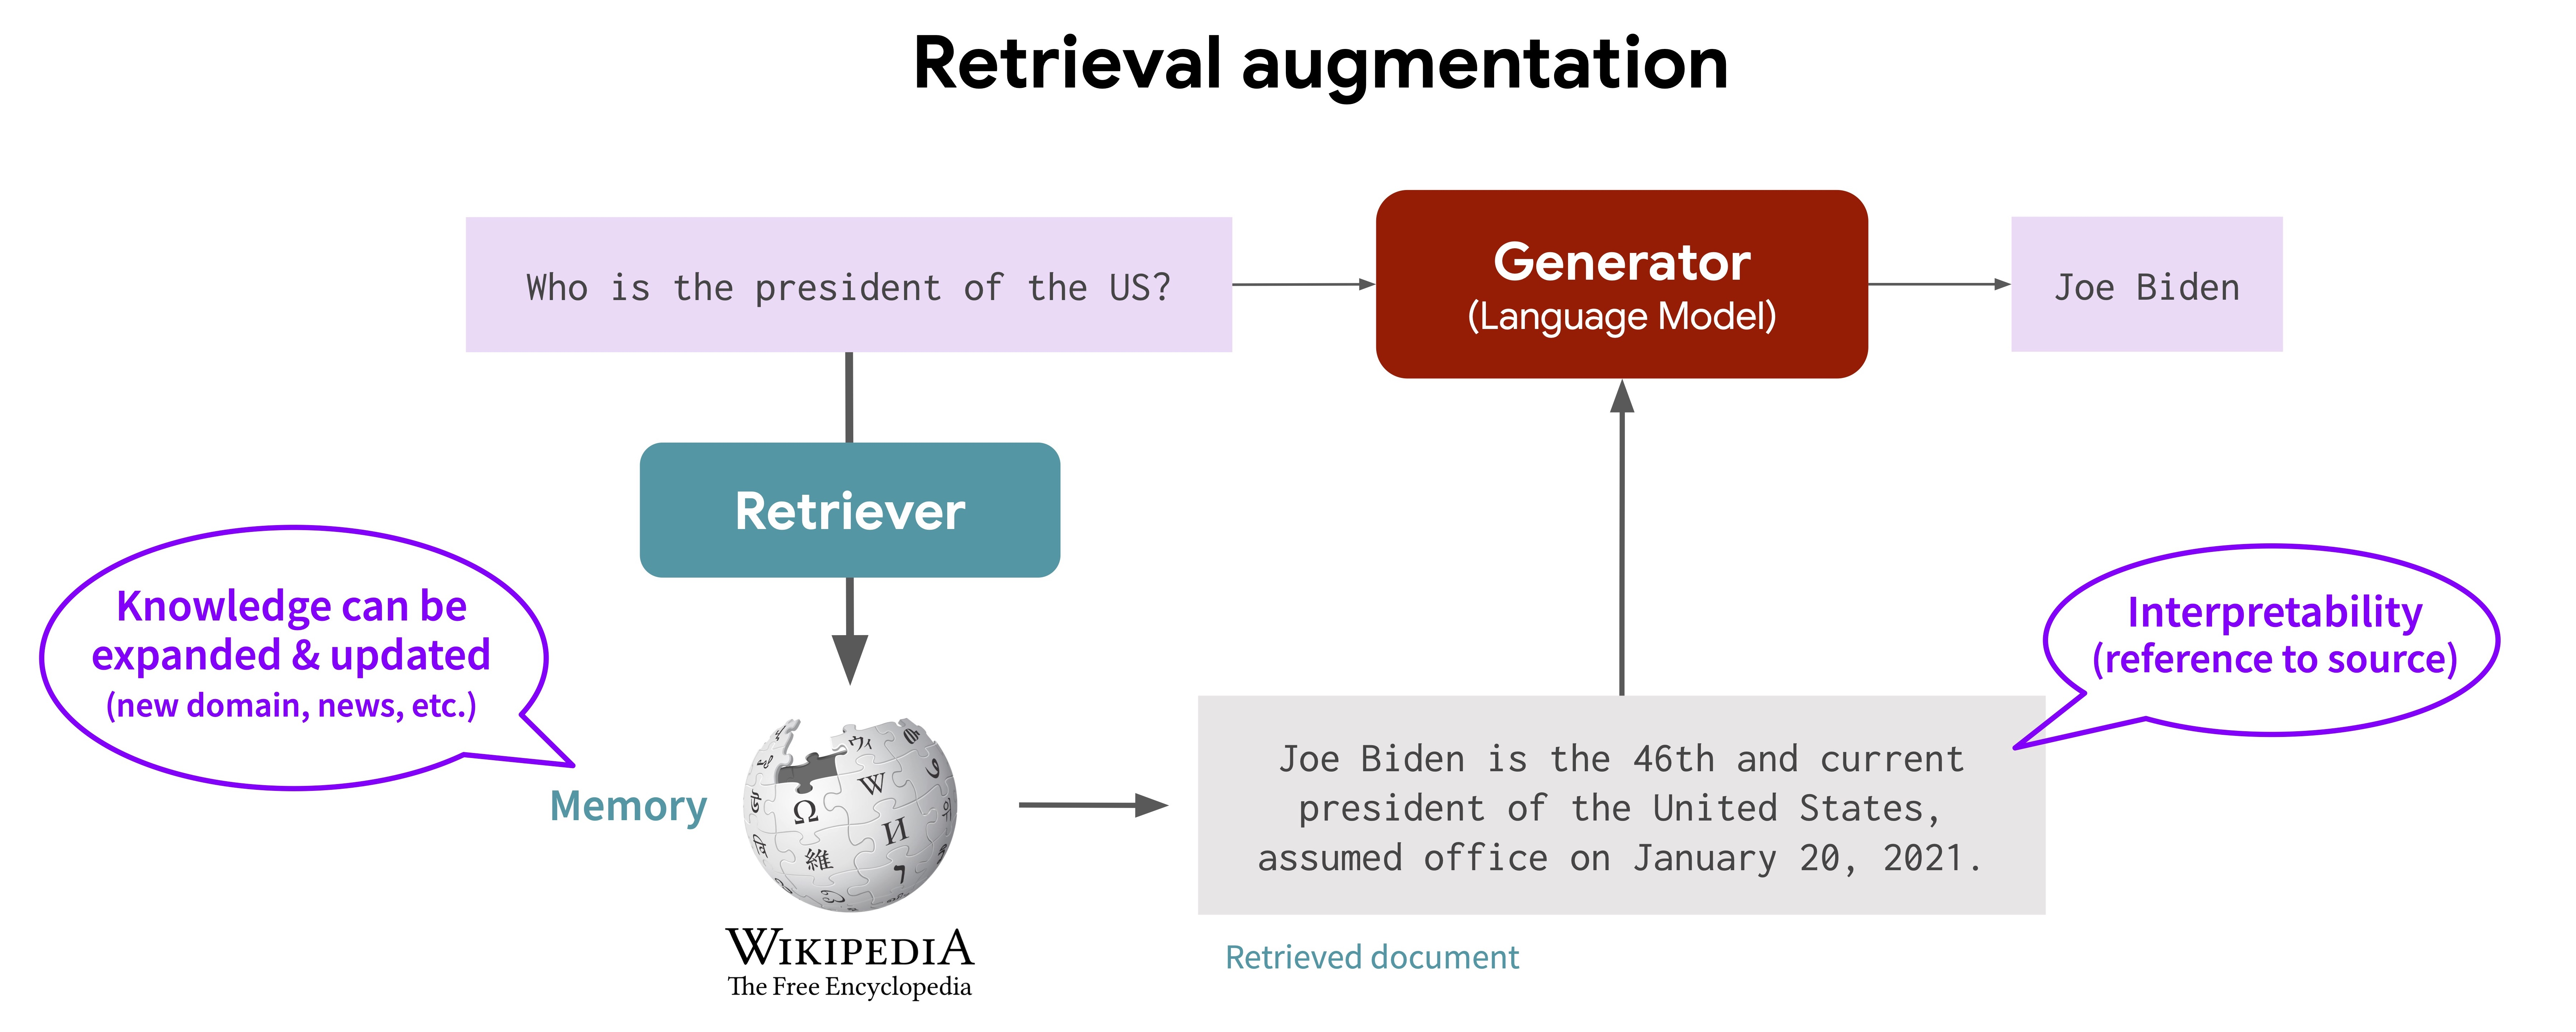
\includegraphics[width=0.8\textwidth]{related-work/images/rag.png}
    \caption{Illustration of two-stage pipeline in retrieval-augmented generation}
    \label{fig:rag}
\end{figure}
A recent line of work \cite{lewis2020retrieval} has proposed to unify the retriever and the LLM in a single end-to-end model, which can jointly learn to retrieve and generate, which combines a pre-trained language model (PLM), BART, with a Dense Passage Retriever (DPR) following the Bi-encoder architecture. This model can use the input sequence to retrieve relevant passages from Wikipedia and use them as additional context when generating the output sequence.

\section{Graph reasoning}
Graph reasoning is a technique that uses knowledge graphs to enhance the reasoning capabilities of language models. Knowledge graphs are structured representations of entities and their relations, which can provide rich semantic information. Graph reasoning can leverage the graph structure and the logic rules to infer new knowledge, answer complex queries, and discover implicit relationships. Some of the related works that use graph reasoning for knowledge-aware question answering.\\\\
 \textbf{Multi-hop graph relation network} \cite{feng-etal-2020-scalable}: This research proposes a knowledge-aware approach that equips pre-trained language models with a multi-hop relational reasoning module. It performs multi-hop, multi-relational reasoning over subgraphs extracted from external knowledge graphs. The proposed reasoning module unifies path-based reasoning methods and graph neural networks to achieve better interpretability and scalability.\\\\
\textbf{QA-GNN} \cite{yasunaga-etal-2021-qa}: This work presents an end-to-end question answering model that jointly reasons over the knowledge from pre-trained language models and knowledge graphs through graph neural networks. The model addresses two challenges: identifying relevant knowledge from large knowledge graphs, and performing joint reasoning over the QA context and knowledge graph. It uses relevance scoring to estimate the importance of knowledge graph nodes relative to the given QA context, and connects the QA context and knowledge graph to form a joint graph, mutually updating their representations through graph-based message passing
\section{Discussion}
In this chapter, we have seen three distinct approaches to enhance the capabilities of Large Language Models. The first approach, fine-tuning Large Language Models, adapts a pre-trained model to a specific domain or task. This method can improve the model's performance in the targeted domain or task and leverage the general knowledge of the pre-trained language model. However, it can be costly in terms of computational resources and data requirements, and may lead to catastrophic forgetting or poor generalization to out-of-domain scenarios.\\\\
The second approach, retrieval-augmented generation, combines a pre-trained language model with a dense retriever that selects relevant information from a large corpus. This method can address the factuality issue of the Large Language Models, efficiently access and integrate external knowledge sources without fine-tuning. However, retrieval-augmented generation may have difficulty exploring a vast range of documents, especially if they are diverse, noisy, or outdated. Retrieval-augmented generation may also miss important information that is not explicitly stated in the documents.\\\\
The third approach, graph reasoning leverages knowledge graphs to enhance the reasoning capabilities of pretrained language models. While knowledge graphs offer rich semantic information through structured representations of entities and relations, effectively integrating this information poses significant challenges. These challenges include identifying relevant knowledge within large knowledge graphs, performing joint reasoning over both natural language and graph inputs, and inferring implicit knowledge not explicitly stated in the graph.\\\\
Inspired by the strengths and limitations of existing approaches, this project aims to develop a method that efficiently and accurately augments the knowledge of a Large Language Model. We recognize the potential of knowledge graph embedding to address these challenges. Knowledge graph embedding compactly represents entities and relations as vectors, capturing their semantic relationships and enabling efficient knowledge integration within the LLM framework. This approach allows us to leverage the rich information contained in knowledge graphs while mitigating the challenges of missing or implicit knowledge that hinder other methods.

% \input{technologies/front-end-dev}
% \input{technologies/back-end-dev}
% \input{technologies/database-management-system}
% \input{technologies/recommendation-system}